% Options for packages loaded elsewhere
\PassOptionsToPackage{unicode}{hyperref}
\PassOptionsToPackage{hyphens}{url}
%
\documentclass[
  ,jou,floatsintext]{apa6}
\usepackage{amsmath,amssymb}
\usepackage{lmodern}
\usepackage{iftex}
\ifPDFTeX
  \usepackage[T1]{fontenc}
  \usepackage[utf8]{inputenc}
  \usepackage{textcomp} % provide euro and other symbols
\else % if luatex or xetex
  \usepackage{unicode-math}
  \defaultfontfeatures{Scale=MatchLowercase}
  \defaultfontfeatures[\rmfamily]{Ligatures=TeX,Scale=1}
\fi
% Use upquote if available, for straight quotes in verbatim environments
\IfFileExists{upquote.sty}{\usepackage{upquote}}{}
\IfFileExists{microtype.sty}{% use microtype if available
  \usepackage[]{microtype}
  \UseMicrotypeSet[protrusion]{basicmath} % disable protrusion for tt fonts
}{}
\makeatletter
\@ifundefined{KOMAClassName}{% if non-KOMA class
  \IfFileExists{parskip.sty}{%
    \usepackage{parskip}
  }{% else
    \setlength{\parindent}{0pt}
    \setlength{\parskip}{6pt plus 2pt minus 1pt}}
}{% if KOMA class
  \KOMAoptions{parskip=half}}
\makeatother
\usepackage{xcolor}
\usepackage{graphicx}
\makeatletter
\def\maxwidth{\ifdim\Gin@nat@width>\linewidth\linewidth\else\Gin@nat@width\fi}
\def\maxheight{\ifdim\Gin@nat@height>\textheight\textheight\else\Gin@nat@height\fi}
\makeatother
% Scale images if necessary, so that they will not overflow the page
% margins by default, and it is still possible to overwrite the defaults
% using explicit options in \includegraphics[width, height, ...]{}
\setkeys{Gin}{width=\maxwidth,height=\maxheight,keepaspectratio}
% Set default figure placement to htbp
\makeatletter
\def\fps@figure{htbp}
\makeatother
\setlength{\emergencystretch}{3em} % prevent overfull lines
\providecommand{\tightlist}{%
  \setlength{\itemsep}{0pt}\setlength{\parskip}{0pt}}
\setcounter{secnumdepth}{-\maxdimen} % remove section numbering
% Make \paragraph and \subparagraph free-standing
\ifx\paragraph\undefined\else
  \let\oldparagraph\paragraph
  \renewcommand{\paragraph}[1]{\oldparagraph{#1}\mbox{}}
\fi
\ifx\subparagraph\undefined\else
  \let\oldsubparagraph\subparagraph
  \renewcommand{\subparagraph}[1]{\oldsubparagraph{#1}\mbox{}}
\fi
\newlength{\cslhangindent}
\setlength{\cslhangindent}{1.5em}
\newlength{\csllabelwidth}
\setlength{\csllabelwidth}{3em}
\newlength{\cslentryspacingunit} % times entry-spacing
\setlength{\cslentryspacingunit}{\parskip}
\newenvironment{CSLReferences}[2] % #1 hanging-ident, #2 entry spacing
 {% don't indent paragraphs
  \setlength{\parindent}{0pt}
  % turn on hanging indent if param 1 is 1
  \ifodd #1
  \let\oldpar\par
  \def\par{\hangindent=\cslhangindent\oldpar}
  \fi
  % set entry spacing
  \setlength{\parskip}{#2\cslentryspacingunit}
 }%
 {}
\usepackage{calc}
\newcommand{\CSLBlock}[1]{#1\hfill\break}
\newcommand{\CSLLeftMargin}[1]{\parbox[t]{\csllabelwidth}{#1}}
\newcommand{\CSLRightInline}[1]{\parbox[t]{\linewidth - \csllabelwidth}{#1}\break}
\newcommand{\CSLIndent}[1]{\hspace{\cslhangindent}#1}
\ifLuaTeX
\usepackage[bidi=basic]{babel}
\else
\usepackage[bidi=default]{babel}
\fi
\babelprovide[main,import]{english}
% get rid of language-specific shorthands (see #6817):
\let\LanguageShortHands\languageshorthands
\def\languageshorthands#1{}
% Manuscript styling
\usepackage{upgreek}
\captionsetup{font=singlespacing,justification=justified}

% Table formatting
\usepackage{longtable}
\usepackage{lscape}
% \usepackage[counterclockwise]{rotating}   % Landscape page setup for large tables
\usepackage{multirow}		% Table styling
\usepackage{tabularx}		% Control Column width
\usepackage[flushleft]{threeparttable}	% Allows for three part tables with a specified notes section
\usepackage{threeparttablex}            % Lets threeparttable work with longtable

% Create new environments so endfloat can handle them
% \newenvironment{ltable}
%   {\begin{landscape}\centering\begin{threeparttable}}
%   {\end{threeparttable}\end{landscape}}
\newenvironment{lltable}{\begin{landscape}\centering\begin{ThreePartTable}}{\end{ThreePartTable}\end{landscape}}

% Enables adjusting longtable caption width to table width
% Solution found at http://golatex.de/longtable-mit-caption-so-breit-wie-die-tabelle-t15767.html
\makeatletter
\newcommand\LastLTentrywidth{1em}
\newlength\longtablewidth
\setlength{\longtablewidth}{1in}
\newcommand{\getlongtablewidth}{\begingroup \ifcsname LT@\roman{LT@tables}\endcsname \global\longtablewidth=0pt \renewcommand{\LT@entry}[2]{\global\advance\longtablewidth by ##2\relax\gdef\LastLTentrywidth{##2}}\@nameuse{LT@\roman{LT@tables}} \fi \endgroup}

% \setlength{\parindent}{0.5in}
% \setlength{\parskip}{0pt plus 0pt minus 0pt}

% Overwrite redefinition of paragraph and subparagraph by the default LaTeX template
% See https://github.com/crsh/papaja/issues/292
\makeatletter
\renewcommand{\paragraph}{\@startsection{paragraph}{4}{\parindent}%
  {0\baselineskip \@plus 0.2ex \@minus 0.2ex}%
  {-1em}%
  {\normalfont\normalsize\bfseries\itshape\typesectitle}}

\renewcommand{\subparagraph}[1]{\@startsection{subparagraph}{5}{1em}%
  {0\baselineskip \@plus 0.2ex \@minus 0.2ex}%
  {-\z@\relax}%
  {\normalfont\normalsize\itshape\hspace{\parindent}{#1}\textit{\addperi}}{\relax}}
\makeatother

% \usepackage{etoolbox}
\makeatletter
\patchcmd{\HyOrg@maketitle}
  {\section{\normalfont\normalsize\abstractname}}
  {\section*{\normalfont\normalsize\abstractname}}
  {}{\typeout{Failed to patch abstract.}}
\patchcmd{\HyOrg@maketitle}
  {\section{\protect\normalfont{\@title}}}
  {\section*{\protect\normalfont{\@title}}}
  {}{\typeout{Failed to patch title.}}
\makeatother

\usepackage{xpatch}
\makeatletter
\xapptocmd\appendix
  {\xapptocmd\section
    {\addcontentsline{toc}{section}{\appendixname\ifoneappendix\else~\theappendix\fi\\: #1}}
    {}{\InnerPatchFailed}%
  }
{}{\PatchFailed}
\usepackage{dblfloatfix}


\usepackage{csquotes}
\ifLuaTeX
  \usepackage{selnolig}  % disable illegal ligatures
\fi
\IfFileExists{bookmark.sty}{\usepackage{bookmark}}{\usepackage{hyperref}}
\IfFileExists{xurl.sty}{\usepackage{xurl}}{} % add URL line breaks if available
\urlstyle{same} % disable monospaced font for URLs
\hypersetup{
  pdftitle={Faith in Reason: developing a survey measure of belief in the rationality of others},
  pdfauthor={Tom Stafford1, Junyan Zhu2, \& Katharine Dommett2},
  pdflang={en-EN},
  hidelinks,
  pdfcreator={LaTeX via pandoc}}

\title{Faith in Reason: developing a survey measure of belief in the rationality of others}
\author{Tom Stafford\textsuperscript{1}, Junyan Zhu\textsuperscript{2}, \& Katharine Dommett\textsuperscript{2}}
\date{}


\shorttitle{Faith in Reason}

\authornote{

For the purpose of open access, the author has applied a Creative Commons Attribution (CC BY) licence to any Author Accepted Manuscript version arising.

Document prepared with RMarkdown (Allaire et al., 2020) and papaja (Aust \& Barth, 2020). CRediT (Contributor Roles Taxonomy) autogenerated using Tenzing (Holcombe, Kovacs, Aust, \& Aczel, 2020). Template is available here \href{https://github.com/tomstafford/rmarkdown_apa}{github.com/tomstafford/rmarkdown\_apa}

The authors made the following contributions. Tom Stafford: Conceptualization, Data curation, Formal analysis, Funding acquisition, Methodology, Visualization, Writing - original draft, Writing - review \& editing; Junyan Zhu: Conceptualization, Data curation, Formal analysis, Methodology, Writing - review \& editing; Katharine Dommett: Conceptualization, Funding acquisition, Methodology, Writing - review \& editing.

Correspondence concerning this article should be addressed to Tom Stafford, Department of Psychology, University of Sheffield, Sheffield, UK. E-mail: \href{mailto:t.stafford@sheffield.ac.uk}{\nolinkurl{t.stafford@sheffield.ac.uk}}

}

\affiliation{\vspace{0.5cm}\textsuperscript{1} Department of Psychology, University of Sheffield, UK\\\textsuperscript{2} Department of Politics and International Relations, University of Sheffield, UK}

\note{\textcolor{red}{Draft, not for circulation 2023-05-03}}

\abstract{%
What we believe about other people matters. It is not enough that others \emph{are} trustworthy, reasonable or well intentioned. Successful coordination, as well as individual wellbeing, benefit when we also \emph{perceive} others as trustworthy, reasonable or well intentioned. While standard measures of trust and benevolence exist, there is no standard measure of the generalised belief in the rationality or reasonableness of other people. Here, we present the development and testing of a scale to directly measure this attitude. Using a representative sample of 1869 UK adults, we test dimensionality and consistency of the scale items. We show that the refined, six-item, scale is associated with, but not entirely determined by, generalised trust in other people. Our ``Faith in Reason'' scale shows large individual differences, but the average tendency is slightly on the side of endorsing, rather than rejecting, sentiments such as ``The typical person is often irrational''.
}



\begin{document}
\maketitle

\hypertarget{introduction}{%
\section{Introduction}\label{introduction}}

\hypertarget{rationality}{%
\subsection{Rationality}\label{rationality}}

\begin{quote}
\emph{All our dignity consists then in thought. By it we must elevate ourselves, and not by space and time which we cannot fill. Let us endeavour then to think well; this is the principle of morality.}
Pascal (1669/1910)
\end{quote}

The nature of human reason is a perennial topic. Human rationality has often been praised (``Man is but a reed, the most feeble thing in nature, but he is a thinking reed,'' Pascal, 1669/1910), but so have its failures condemned been by many different thinkers.

An influential account of human reasoning is provided by the heuristics and biases programme (Kahneman, Slovic, \& Tversky, 1982), which uses the ideal of economic rationality as a standard to define actual human reasoning against. From this perspective human reasoning appears riddled with biases, but much of this effect is due to the adoption of the standards of utility theory, formal logic and precise statistical reasoning against which to define error. Critics have questions the appropriateness of these standards (e.g. Gigerenzer \& Gaissmaier, 2011). The logic of controlled experiments allows researchers to isolate and emphasise quirks in human reasoning, while backgrounding reason-responsiveness (Stafford, 2014). Accordingly, the psychology literature may overemphasise the role of error, bias and motivated reasoning (Stafford, 2020). The debate has been so heated in the cognitive sciences that `Rationality Wars' (Samuels, Stich, \& Bishop, 2002) have been declared over the definition of rationality that might reasonably used as a standard against which to judge human reasoning.

Mercier and Sperber's (2011) Argumentative Theory of Reason provides an interactionist, rather than individualist account of human reasoning, which emphasises the social context in which human reasoning evolved. This account suggests, among other things, the importance of dialogue based argumentation in changing beliefs (Brand \& Stafford, 2022; Karadzhov, Stafford, \& Vlachos, 2022) and the validity of incorporating social factors like the status, trustworthiness or expertise of a source of information in the reasoning process (Eiser, Stafford, Henneberry, \& Catney, 2009).

\hypertarget{criteria-of-reason}{%
\subsection{Criteria of reason}\label{criteria-of-reason}}

So rationality is not a unitary concept, nor one around which there is consensus on the definition of, despite the way it is often evoked in discussion (and particularly in discussion of its negation e.g.~``they are being irrational''). That said, core features of rationality have been proposed, and it may be possible to test these as aspects of the `folk theory' of rationality that exists in the common understanding.

Two primary criteria are `\textbf{correspondence}', where beliefs are aligned with reality (in the form of the state of the world or their behaviour), and `\textbf{coherence}', where beliefs are aligned with each other (i.e.~consistent, but see Sommer, Musolino, \& Hemmer, 2022). For more on corresponence and coherance see Dawson and Gregory (2009).

Another criteria of rationalty which can be identified is \textbf{insight} into your own beliefs and how they guide behaviour. The rhetorical power of certain celebrated demonstrations of irrationality (e.g. Nisbett \& Wilson, 1977) relies on the surprise that people can act, supposedly, unaware of the causes of their behaviour (but see Stafford, 2020).

Finally, susceptibility to \textbf{influence} is a key aspect of rationality (Mercier, 2020). This can be positively construed - to be rational is to be responsive to reasons, persuadable by evidence and so on. And it can be negative construed - to be irrational is to be gullible, or stubborn in the face of good reasons to change your mind.

So core features of rationality include coherence, correspondence, susceptibility to influence and insight into causes of ones actions. The extent to which these features form a coherent whole in the minds of the general public, and can meaningfully be asked about questions about is a primary question of this paper.

\hypertarget{consequence-of-a-lack-of-faith-in-reason}{%
\subsection{Consequence of a lack of faith in reason}\label{consequence-of-a-lack-of-faith-in-reason}}

Investigating folk conceptions of rationality is not just interesting in its own right, individual's beliefs about the rationality of others may be important for a number of other core beliefs and behaviours.

\hypertarget{second-order-effects-of-disinformation}{%
\subsubsection{Second order effects of disinformation}\label{second-order-effects-of-disinformation}}

The generalised belief that others are well informed and reasonable is foundational to democracy. Recent concerns around misinformation may have second order effects, undermining democracy not by generating a misinformed populace, but by generating a populace that believes others are misunformed or unreasonable (Karpf, 2019). Alarmism around misinformation may potentially lower trust in institutions (Hoes, Clemm von Hohenberg, Gessler, Wojcieszak, \& Qian, 2022), increase skepticism about democracy (Jungherr \& Rauchfleisch, 2022; Nisbet, Mortenson, \& Li, 2021), or foster calls of tighter media regulation (Lee, 2021). Altay and Acerbi (2023) have shown that the threat of misinformation is directly related to the perceptions of others' gullibility.

\hypertarget{third-person-effect}{%
\subsubsection{Third person effect}\label{third-person-effect}}

There is an established literature of the perception of media influence on others (Perloff, 2002; Sun, Pan, \& Shen, 2008). The `third person effect', proposed by Davison (1983), is the phenomenon whereby many people believe others are more susceptible to influence than themselves. The third person effect was proposed as a root cause of censorship instincts and this has been confirmed by subsequent empirical investigations (Feng \& Guo, 2012; Olshansky \& Landrum, 2020).

Two caveats around the third person effect. Lyons (2022) has recently argued that - for many people - a third person effect of greater media influence on others rather than the self will be an accurate perception. Chung and Moon (2016) have argued that the driving factor in many so-called third person effects is the perception of others (as highly influenced), rather than the discrepancy with first person perception per se.

\hypertarget{generalised-trust-value-of-democracy}{%
\subsection{Generalised trust \& value of democracy}\label{generalised-trust-value-of-democracy}}

Generalised trust is the belief that, `most people can be trusted' (Brehm \& Rahn, 1997; Paxton, 1999). It is reflected in standard items in long running time series surveys such as the World Values Survey (Inglehart \& Team, 2023) an the General Social Survey (General Social Survey Team, 2023). Generalised trust is an aspect of social capital, broadly conceived (Putnam, 2000) and as such as an important aspect of wellbeing and the health of society (Cohn, Maréchal, Tannenbaum, \& Zünd, 2019). Given the recognised importance of generalised trust, it is natural to ask how other beliefs feed into this belief. Why do we trust others? Do we trust them intellectually as well as morally? Do we think other people are able to work things out for themselves, to display good judgement? Do we trust the typical person to avoid being manipulated, to respond to arguments, to reason their way to good enough decisions? In short, is generalised trust informed by beliefs about the rationality or reasonableness of others?

Similarly, attitudes to demoracy may mutually inform beliefs about the reasonableness of one's fellow citizens. One standardised measure of attitude to democracy is the item from the World Values Survey (Inglehart \& Team, 2023) which asks `How important is it for you to live in a country that is governed democratically?'.

\hypertarget{lack-of-existing-measures}{%
\subsection{Lack of existing measures}\label{lack-of-existing-measures}}

To our knowledge, no existing scale directly measures belief in reasoning. There are scales which measure related concepts, or concepts which are plausible antecedents or consequences of belief in the reasonableness of our fellow citizens. In addition to the measures of generalised trust discussed above, there are also measures of conspiracy beliefs or mentality (see Swami et al., 2017 for a brief review) including those which explicitly try to distinguish conspiracist from rational skepticism (Stojanov, Bering, \& Halberstadt, 2020; Stojanov \& Halberstadt, 2019). These do not direct assess rationality, and again could be viewed a more alike to measuring a consequence of rationality or a lack of it (i.e.~due to manipulation or credulity).

Some researchers have looked at what they call `cynical beliefs about human nature' (e.g. Stavrova \& Ehlebracht, 2016), but these, again, do not touch on reason or rationality as a cause of cynicism. Instead, scale items are similar to generalised trust/distrust measures.

Other studies have looked at beliefs about human nature (e.g. Furnham, Johnson, \& Rawles, 1985). These have questions which focus on the role of biology, genetics and/or heredity on psychological traits. For example, asking if participants believe personality is entirely caused by a person's genetics. Again, these scales do not directly assess beliefs about human reason, although they do assess beliefs which may plausibly affect beliefs about human reason.

\hypertarget{summary}{%
\subsection{Summary}\label{summary}}

In summary, generalised belief in the rationality or reasonableness of others is interesting in its own right, in relation to longstanding debates in the cognitive sciences about the definition of rationality and due to plausible relation to other atittudes recognised of importance, such as generalised trust. To our knowledge, no scale exists which directly measures this generalised belief. To develop, refine and explore such a scale is the purpose of the current study.

\hypertarget{method}{%
\section{Method}\label{method}}

\hypertarget{sample}{%
\subsection{Sample}\label{sample}}

The questions were asked as part of a larger survey experiment (Zhu, Dommett, \& Stafford, submitted), in which participants were asked to view adverts which appeared on Facebook during the 2019 UK general election. Participants were recruited via the online platform Prolific. In terms of age, gender, regional dispersion and political affiliations participants reflected a representative sample of UK adults. Data was collected on 2022-08-20. Full details are give in Zhu et al. (submitted).

\hypertarget{item-development}{%
\subsection{Item development}\label{item-development}}

In order to develop the scale items, we developed eight items, informed by the debates in cognitive science around the nature of rationality (see introduction). Half of these were positively framed, to reflect endorsement of human's tendency towards rationality and reasonableness. Half were negatively framed, to reflect endorsement of a tendency towards irrationality and unreasonableness. Items, their framing (positive/negative) and the aspect of rationality they were designed to capture are shown in Table \ref{tab:items}.

\begin{table*}[tbp]

\begin{center}
\begin{threeparttable}

\caption{\label{tab:items}Scale item wording}

\begin{tabular}{llll}
\toprule
Item & \multicolumn{1}{c}{Framing} & \multicolumn{1}{c}{Aspect} & \multicolumn{1}{c}{Wording}\\
\midrule
R1 & negative & general & The typical person is often irrational\\
R2 & negative & corresponence & People are often misinformed on important issues\\
R3 & negative & influence & People are too easily manipulated\\
R4 & negative & insight & People often act for reasons they don’t understand or endorse\\
R5 & positive & influence & The average person can be persuaded to change their mind if given good reasons\\
R6 & positive & correspondence & Most people hold accurate views about the world\\
A & NA & ATTN CHECK & For this question please click the middle option, ‘neutral’, to show you are paying attention\\
R7 & positive & coherance & An individual's beliefs about the world are generally coherent\\
R8 & positive & coherance & People's behaviour is generally consistent with their beliefs\\
\bottomrule
\addlinespace
\end{tabular}

\begin{tablenotes}[para]
\normalsize{\textit{Note.} Response was on a 7 point Likert scale from (1 = "Strongly Disagree", 7 = "Strongly Agree"). Items 1,2,3 and 4 reverse coded so that for all items higher scores represented stronger faith in reason.}
\end{tablenotes}

\end{threeparttable}
\end{center}

\end{table*}

In all analyses negatively framed items were reverse coded, so that numerically higher scores always reflect greater endorsement of human rationality, across all items. An attention check item was included in the scale (also shown in Table \ref{tab:items}).

\hypertarget{other-items}{%
\subsection{Other items}\label{other-items}}

Other items we report from the original survey are a measure of generalised trust (`Generally speaking, would you say that most people can be trusted?'), support for democracy (`How important is it for you to live in a country that is governed democratically?') and a measure of percpetion of the Third Person Effect in the context of political advertising. This was calculated as the average response to six linked items about the influence of election advertising on the typical voter, with wording of the form specifically ``Thinking about the impact of political parties' election messages on the typical voter, to what extent do you agree or disagree that it helps to: - Raise their awareness of political issues; Raise their awareness of political candidates or parties; Prompt them to share messages related to the election; Prompt them to vote/ register to vote; Persuade them to change who you are planning to vote for; Influence how they feel about political opponents'. We also report demographic questions (age, sex, education)

\hypertarget{preregistration}{%
\subsection{Preregistration}\label{preregistration}}

Our analysis is supported by formal preregistration of hypothesis and data analyses practices
(OSF pre-registration link: \url{https://osf.io/y9kjg/?view_only=609cd46aab534e4c866c16b3ef29c510}). Note that the bulk of this preregistration concerns the analyses reported in Zhu et al. (submitted).

Preregistration supports the accurate identification of confirmatory versus exploratory analyses. The nature of scale development is necessarily exploratory, but the preregistration allows readers confirm what was intended and expected before data was collected.

\hypertarget{reproducibility}{%
\subsection{Reproducibility}\label{reproducibility}}

Data availability: The analysis code and anonymised response data which supports all results are openly available \url{https://github.com/tomstafford/faithinreason}

This repository contains the files used to generate this report, which is in the form of a `reproducible manuscript', a document which generates the analysis it reports, and so combines sharing, documenting and reporting an analysis in a single set of project files (Allaire et al., 2020 ; Aust \& Barth, 2020). Details of the statistical software packages used can be found in the repository, and via these citations (Aust \& Barth, 2020; Epskamp, Cramer, Waldorp, Schmittmann, \& Borsboom, 2012; H. Golino \& Christensen, 2022; Müller, 2020; Revelle, 2022; Rizopoulos, 2006; Van der Ark, 2007; van der Laken, 2022; Wickham et al., 2019; Xie, 2022).

\hypertarget{results}{%
\section{Results}\label{results}}

\hypertarget{initial-characterisations}{%
\subsection{Initial characterisations}\label{initial-characterisations}}

Our data consist of 1881 participants who completed our online survey. 6 failed an attention check and were removed, leaving a final sample of 1875. Inital inspection suggested that a range of responses were obtained. Table \ref{tab:itemmeans} shows that the first item of the scale received the full range of responses from ``Strongly disagree'' to ``Strongly agree''.

\begin{table}[tbp]

\begin{center}
\begin{threeparttable}

\caption{\label{tab:itemmeans}Summary statistics for each item}

\begin{tabular}{llllll}
\toprule
Item & \multicolumn{1}{c}{mean} & \multicolumn{1}{c}{median} & \multicolumn{1}{c}{min} & \multicolumn{1}{c}{max} & \multicolumn{1}{c}{SD}\\
\midrule
R1 & 4.15 & 4.00 & 1.00 & 7.00 & 1.34\\
R2 & 2.54 & 3.00 & 1.00 & 7.00 & 1.11\\
R3 & 2.55 & 3.00 & 1.00 & 7.00 & 1.07\\
R4 & 2.88 & 3.00 & 1.00 & 7.00 & 1.14\\
R5 & 5.05 & 5.00 & 1.00 & 7.00 & 1.16\\
R6 & 3.54 & 4.00 & 1.00 & 7.00 & 1.23\\
R7 & 4.09 & 4.00 & 1.00 & 7.00 & 1.12\\
R8 & 4.62 & 5.00 & 1.00 & 7.00 & 1.19\\
\bottomrule
\addlinespace
\end{tabular}

\begin{tablenotes}[para]
\normalsize{\textit{Note.} Items 1,2,3 and 4 are reverse coded, so lower scores imply stronger endorsement of the question framing (but lower faith in reason)}
\end{tablenotes}

\end{threeparttable}
\end{center}

\end{table}

\hypertarget{scale-development-assessing-dimensionality-item-selection}{%
\subsection{Scale development: assessing dimensionality \& item selection}\label{scale-development-assessing-dimensionality-item-selection}}

Cronbach's alpha for all eight items is 0.72, which is often taken to reflect good-to-acceptable scale consistency. A leave-one-out procedure suggests that Cronbach's Alpha decreases for omission of all items except item 5, without which the Cronbach's Alpha of the remaining 7 items is 0.78. The caveat to this is that, properly, Cronbach's Alpha should be measured \emph{after} confirmation of unidimensionality.

A conventional method for assessing dimensionality is factor analysis. Figure \ref{fig:factor8} shows the scree plot for the eight items. The result is ambiguous, since there is one main factor but a second factor which falls just below the traditional cut-off an eigenvalue of 1.

\begin{figure}

{\centering 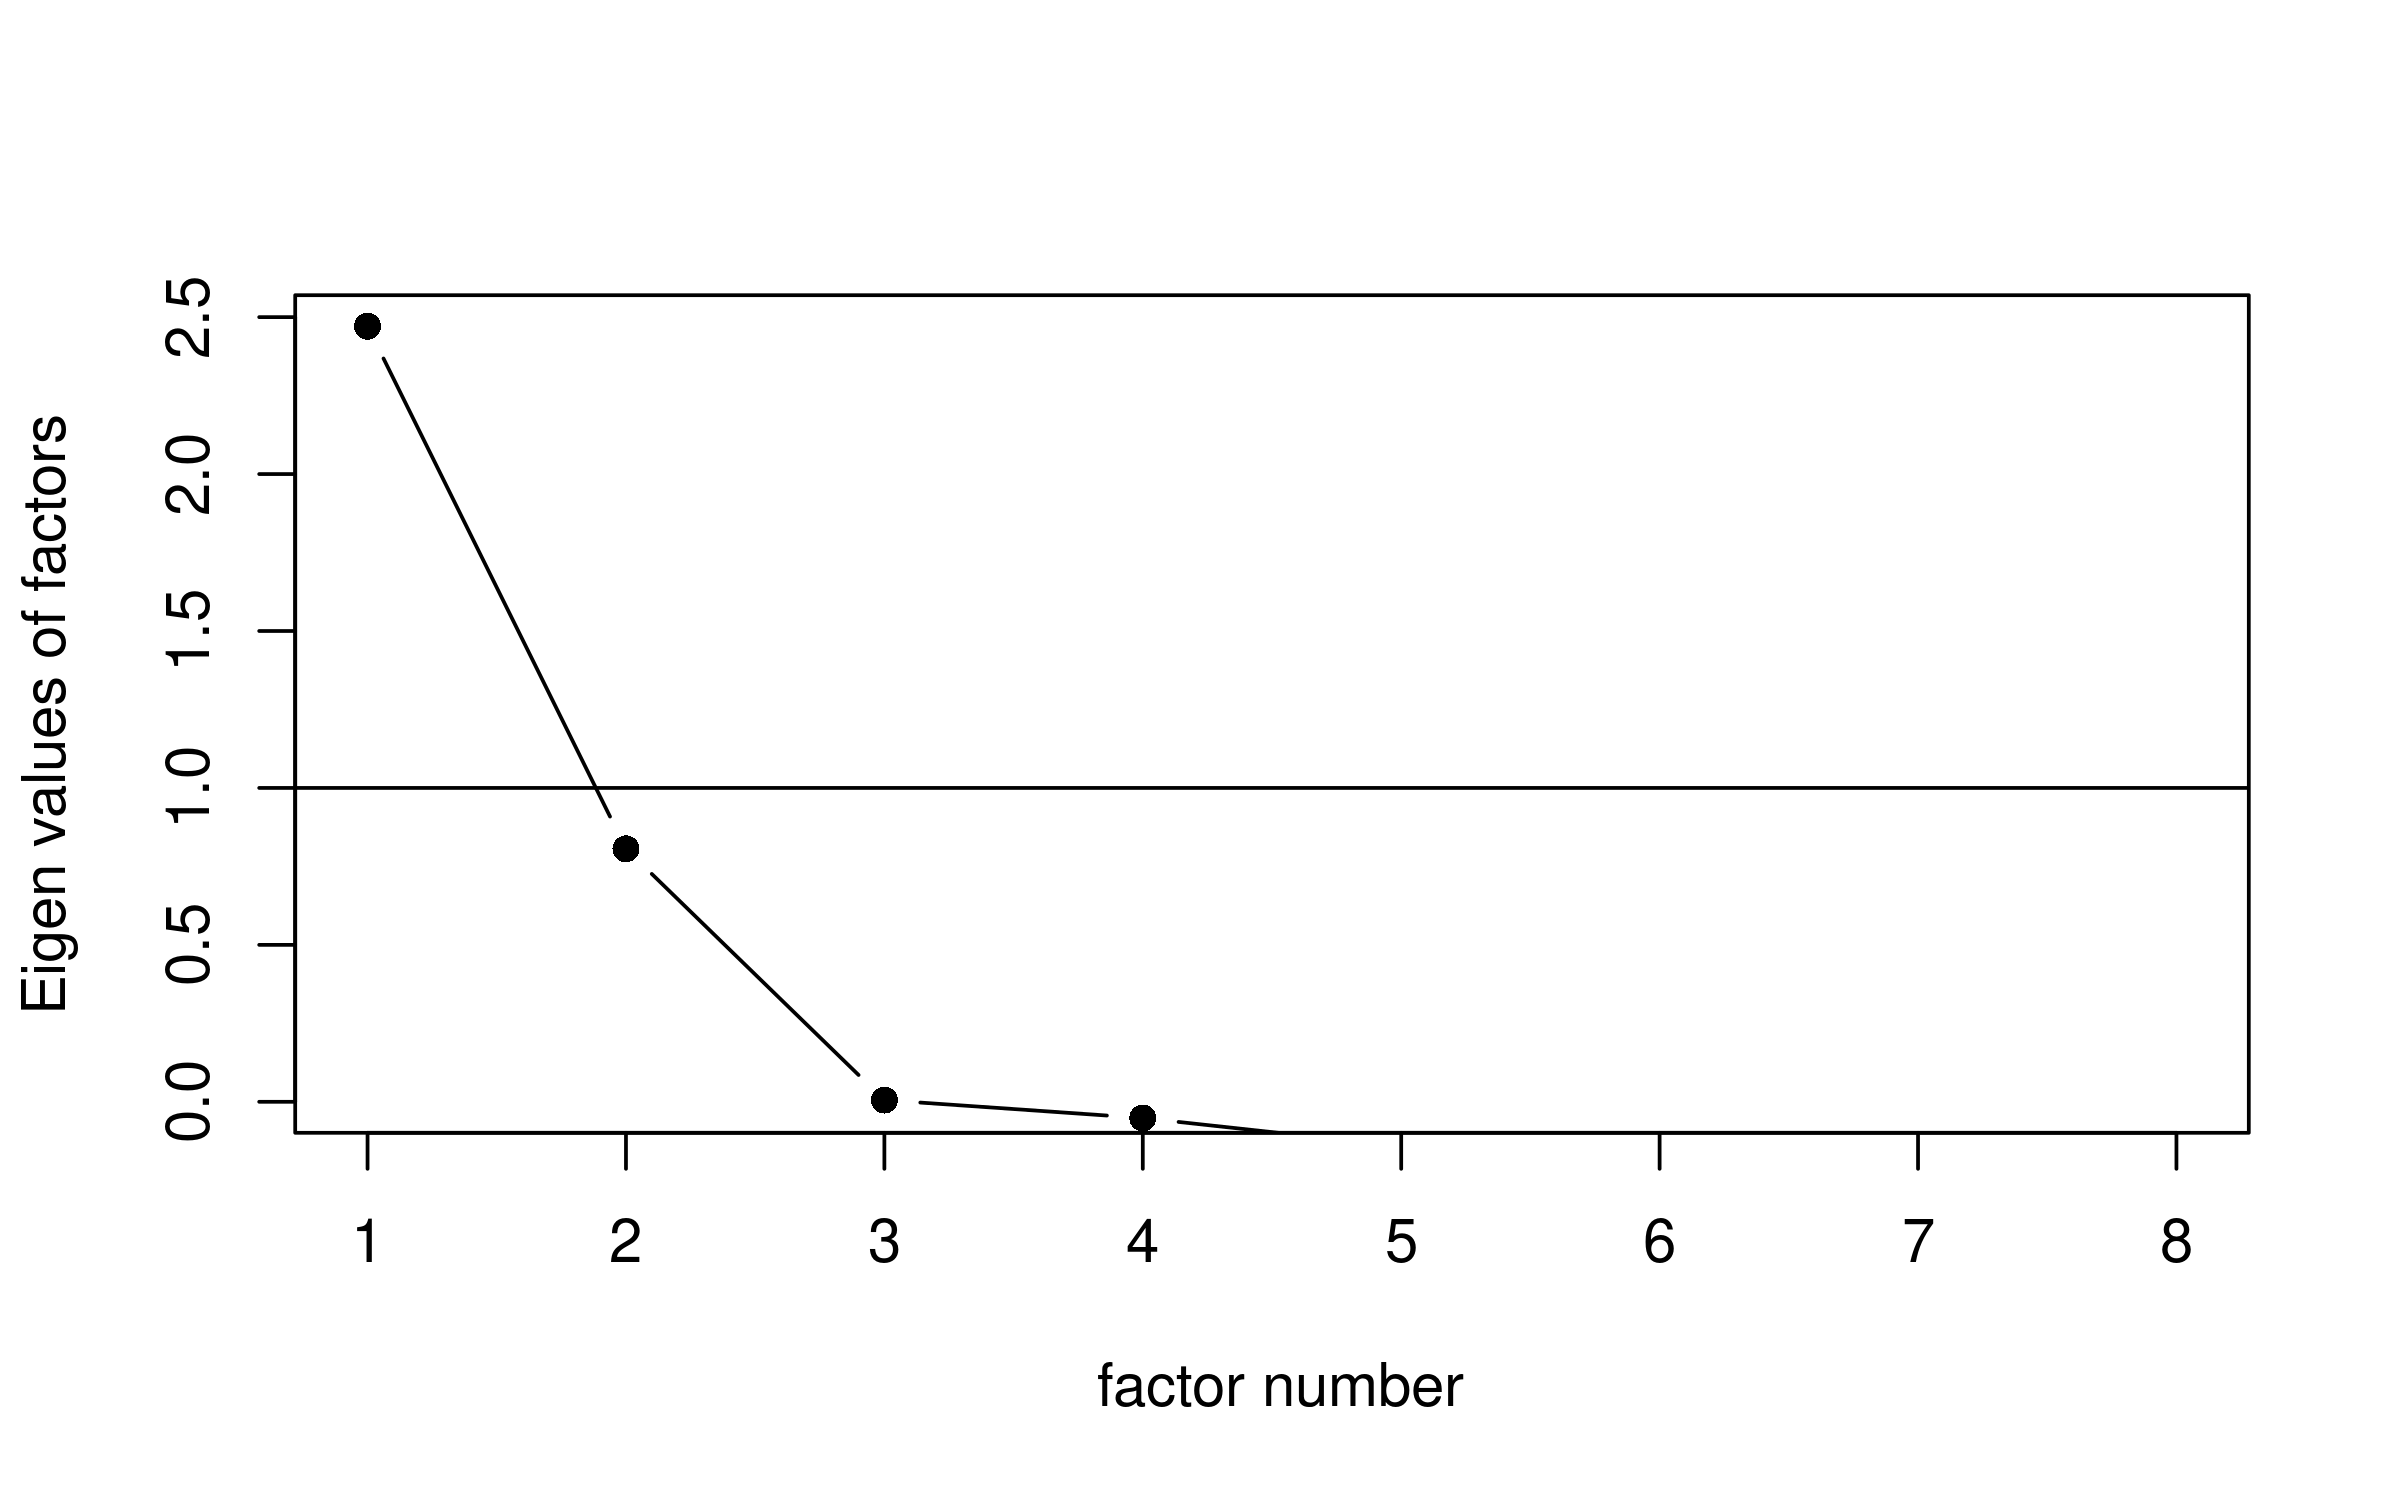
\includegraphics[width=1\linewidth]{plots/reason_scree8} 

}

\caption{Factor analysis for 8 items of the Faith in Reason scale}\label{fig:factor8}
\end{figure}

\hypertarget{mokken-analysis}{%
\subsubsection{Mokken Analysis}\label{mokken-analysis}}

To understand the dimensional structure of our items, we turn to Mokken Analysis, part of the item response theory framework (Sijtsma \& Ark, 2017; Van Schuur, 2011). Very loosely, Mokken analysis tests scale items against a model which assumes that items are monotonically ordered on a single dimension, with some affording higher responses and others affording lower responses, with this item property consistent across participants, who also vary in their propensity to give high or low responses. Violations of this model indicate that items do fit on a single dimension and so should not be combined in the same scale.

In Mokken Analysis, the items with low Loevinger's coefficient of homogeneity (\(H i\)), a criterion for scalability, are dropped. A rule of thumb is that \(H i\) must be higher than 0.3 to be kept in the scale. Applying this criterion suggests items 1 to 4, 6 and 7 should be kept, and 5 and 8 dropped. This yields a scale of six items, with an overall H coefficient of 0.410, indicating a medium-strong scalability.

However, following Sijtsma and Ark (2017) it is possible to explore sensitivity of this result to different thresholds. Accordingly, with a threshold of \(0.35\) Mokken scale analysis supports the grouping of the items into two scales (One, items 1,2,3,4 and Two, items 6,7,8, with item 5 fitting in neither scale). This is consonent with the factor analysis which identified a second factor of below threshold salience.

\hypertarget{exploratory-graph-analysis}{%
\subsubsection{Exploratory graph analysis}\label{exploratory-graph-analysis}}

Exploratory Graph Analysis {[}EGA; H. F. Golino, Shi, et al. (2020);H. F. Golino, Christensen, and Moulder (2020){]} can also be applied to understand dimensional structure in our scale items. EGA allows a visualisation of the network formed by scale items, with items which correlate clustered together. EGA also identifies undelrying `communities' of items.

Figure \ref{fig:egafull} shows an EGA for the 8 potential items. Like the use of leave-of-out Cronbach's alpha and the Mokken scale analysis, this suggests Item 5 is distant from the other items. The EGA identifies two communities, grouping Item 1 with Items 6, 7 and 8 and Items 2,3,4 and 5.

\begin{figure}

{\centering 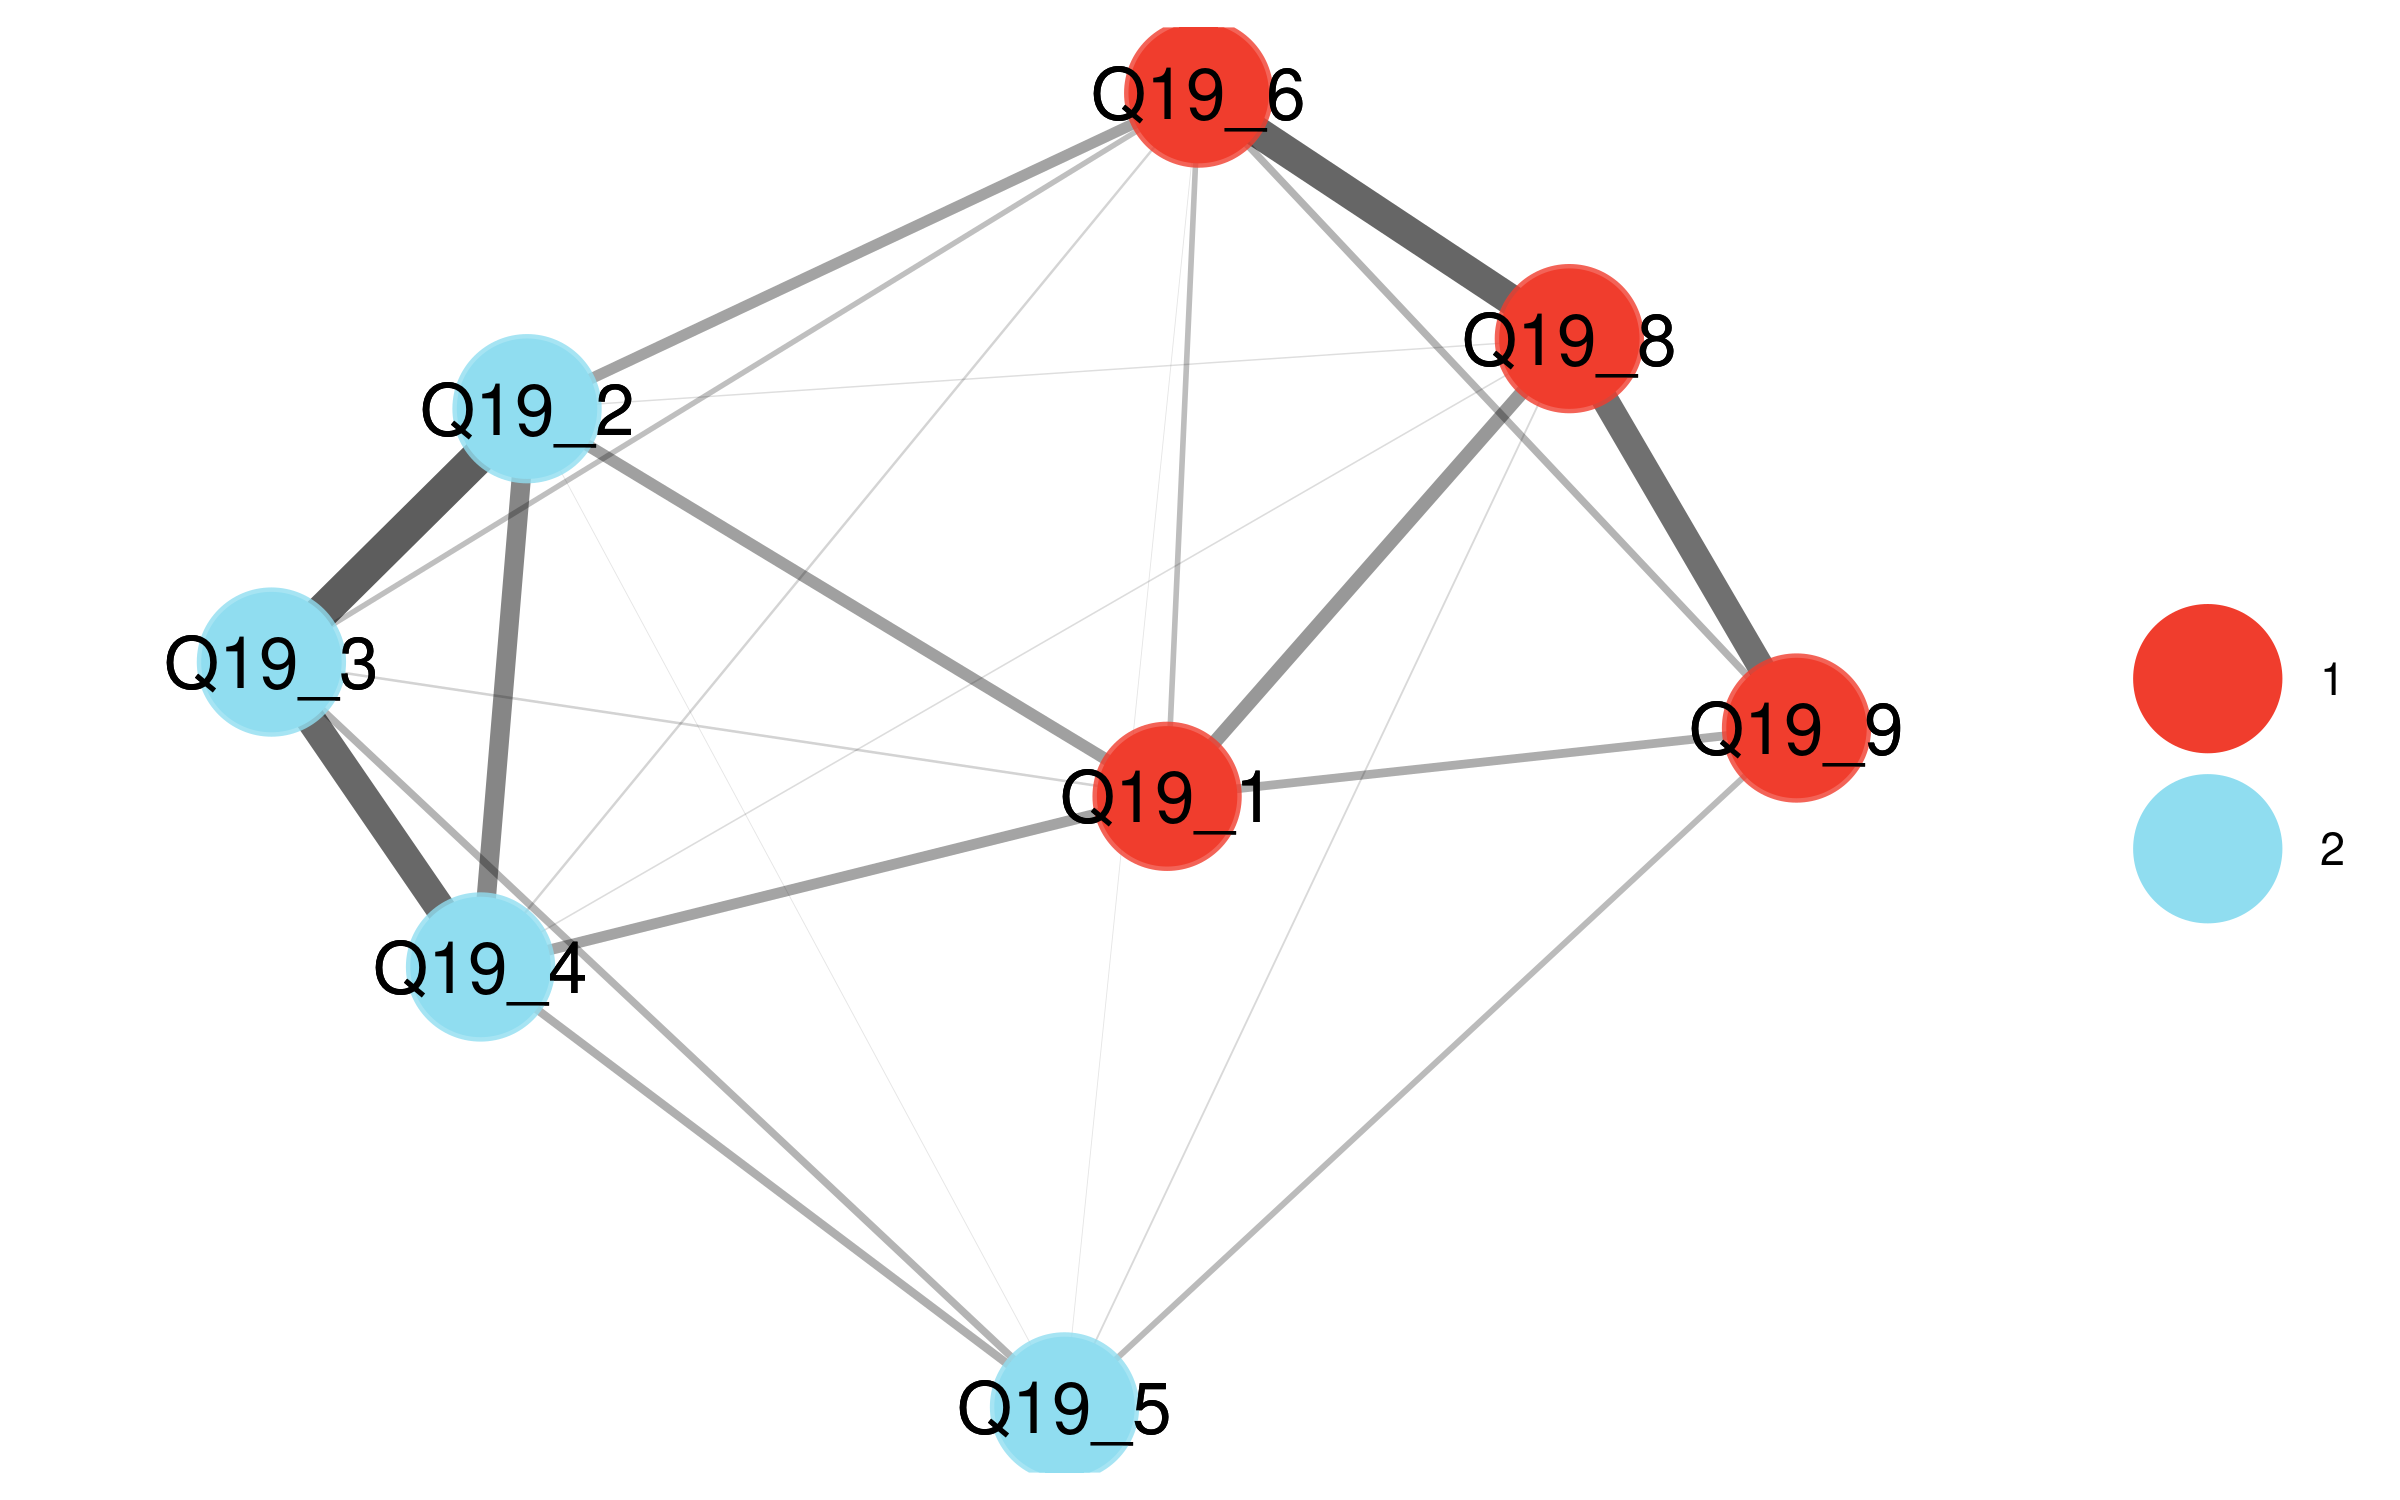
\includegraphics[width=1\linewidth]{plots/reason_ega} 

}

\caption{Exploratory Graph Analysis (EGA) of all items.}\label{fig:egafull}
\end{figure}

\hypertarget{the-faith-in-reason-scale}{%
\subsection{The Faith in Reason scale}\label{the-faith-in-reason-scale}}

Taking these analyses into consideration, we opt to construct a single scale, dropping items 5 and 8. We do this with some hesitation, given that the results from all methods of dimensionality analysis (conventional factor analysis, Mokken scale analysis and EGA) all suggest that a two-dimensional structure may exist (and/or evidence for two dimensional structure is only just sub threshold, depending on how you wish to position the statement ontologically).

\begin{figure}

{\centering 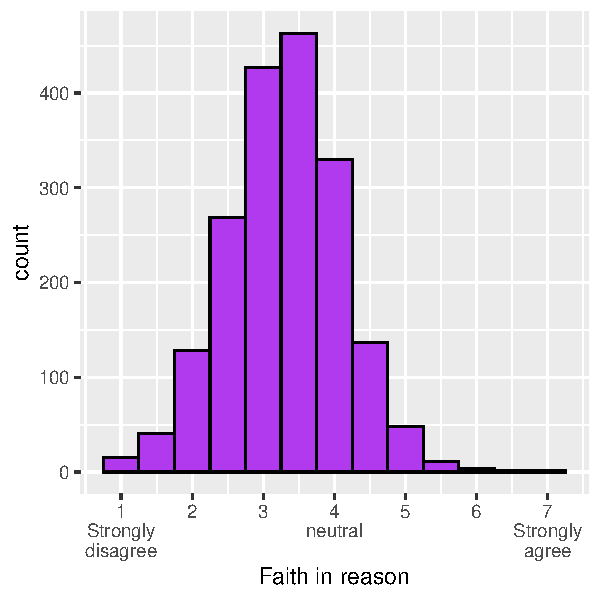
\includegraphics[width=0.75\linewidth]{faithinreason_files/figure-latex/meanhistogram-1} 

}

\caption{Histogram of mean of responses to all rationality items}\label{fig:meanhistogram}
\end{figure}

Averaging across items 1,2,3,4,6 and 7 gives us our Faith in Reason scale. The average score across these six items was 3.29, a summary statistic which suggests that the typical view of other people weighted to being slightly less, rather than slightly more, reasonable. The distribution is shown in Figure \ref{fig:meanhistogram}.

\hypertarget{relation-to-other-variables}{%
\subsection{Relation to other variables}\label{relation-to-other-variables}}

We now turn to ask how scores on this scale are associated with our other measures. Figure \ref{fig:education} shows there is no strong association with level of formal education.

\begin{figure}

{\centering 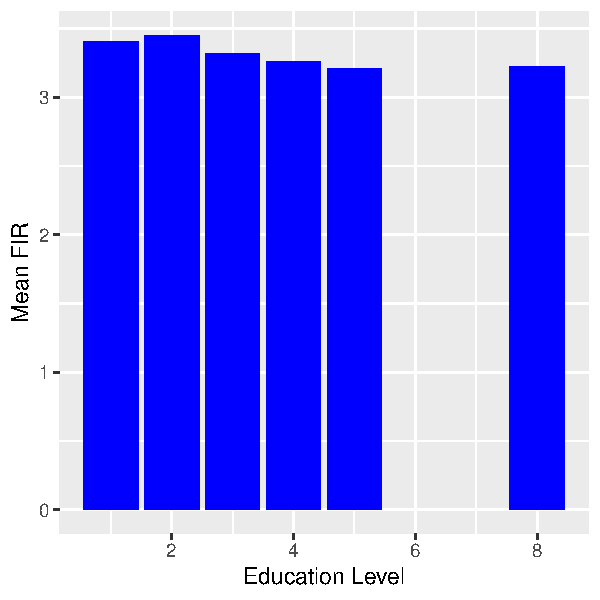
\includegraphics[width=0.75\linewidth]{faithinreason_files/figure-latex/education-1} 

}

\caption{Education level and Faith in Reason}\label{fig:education}
\end{figure}

Figure \ref{fig:democract} shows no strong relation between need for democracy and faith in reason.

\begin{figure}

{\centering 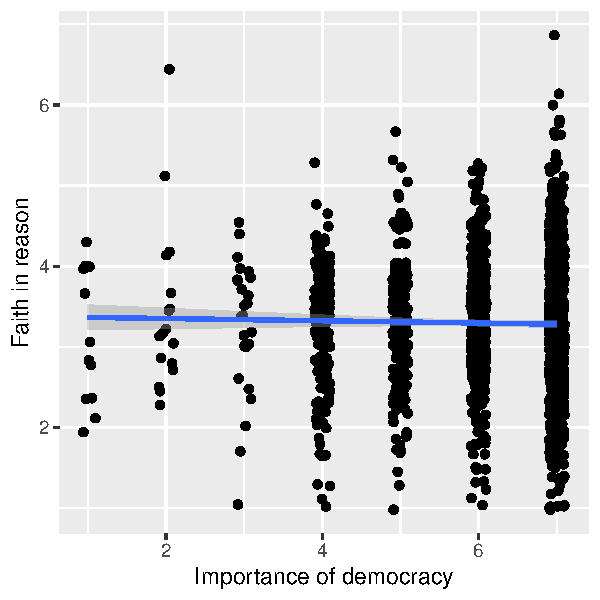
\includegraphics[width=0.75\linewidth]{faithinreason_files/figure-latex/democract-1} 

}

\caption{Scatterplot of Need for Democracy vs Faith in Reason. Linear fit shown. Note 0.1 jitter applied to x-axes values to allow visualisation of point density.}\label{fig:democract}
\end{figure}

Figure \ref{fig:generalisetrust} shows some association between generalised trust and faith in reason.

\begin{figure}

{\centering 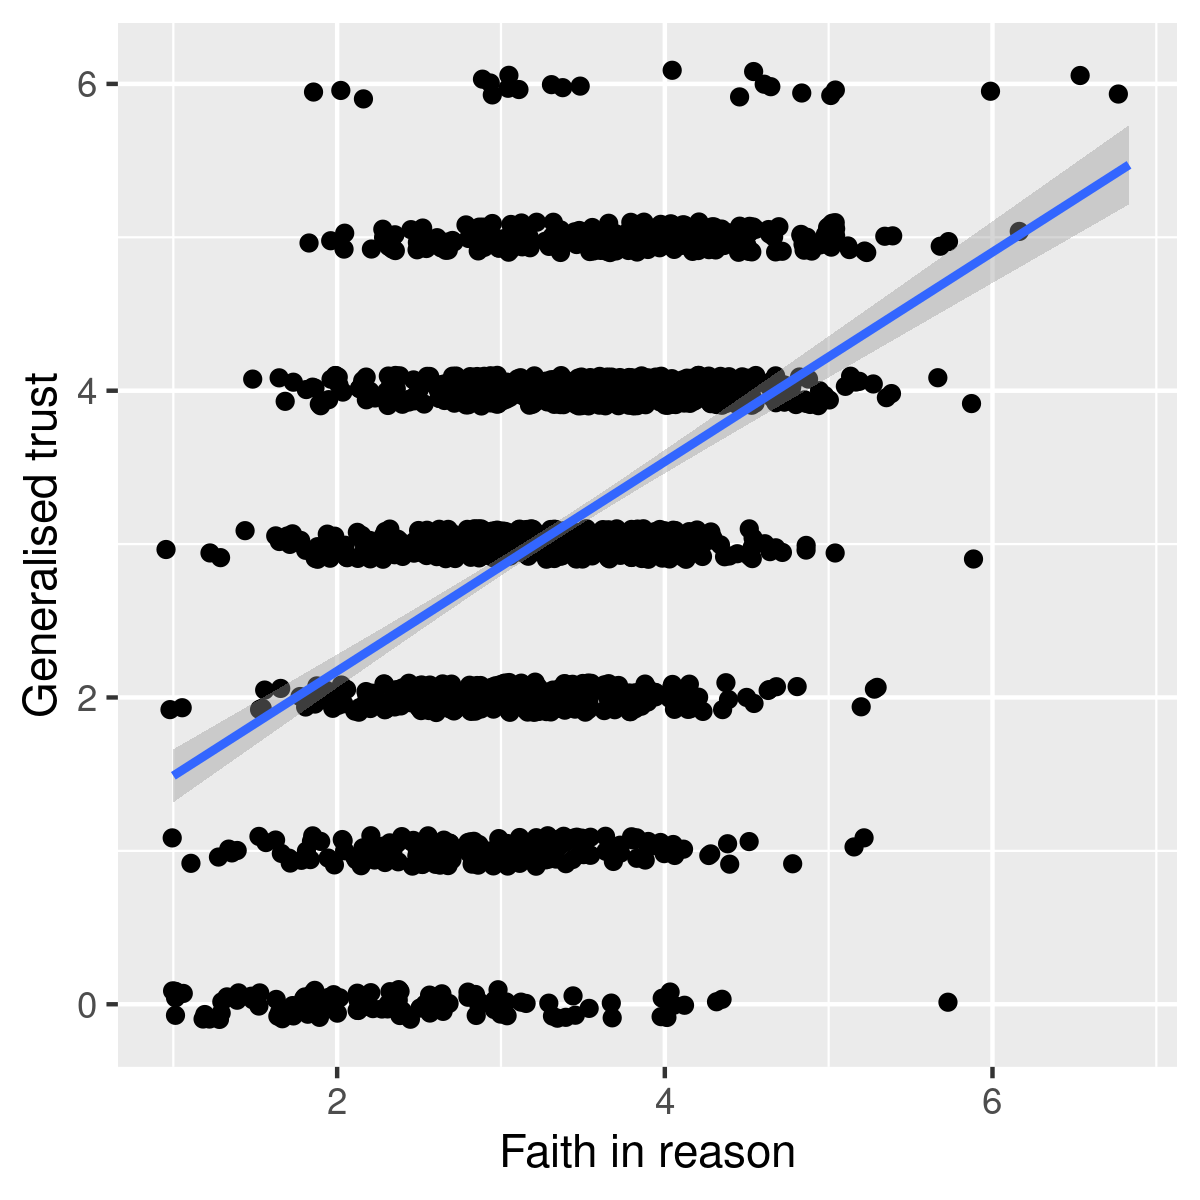
\includegraphics[width=0.75\linewidth]{faithinreason_files/figure-latex/generalisetrust-1} 

}

\caption{Scatterplot of Generalised Trust against Faith in Reason. Linear fit shown. Note 0.1 jitter applied to x-axes values to allow visualisation of point density}\label{fig:generalisetrust}
\end{figure}

There is a convincing lack of association between the Third Person Effect and Faith in Reason (Figure \ref{fig:tpe}).

\begin{table}

\caption{\label{tab:cortable}Correlation Matrix. FIR : Faith in Reason. NfD : Need for Democracy. Trust : Generalised Trust. TPP : Third Person Perception.}
\centering
\begin{tabular}[t]{l|l|l|l|l|l}
\hline
  & FIR  & NfD  & Trust  & Education  & TPP \\
\hline
FIR & 1.00 & -0.02 & 0.40 & -0.09 & -0.00\\
\hline
NfD &  & 1.00 & 0.26 & 0.19 & 0.09\\
\hline
Trust &  &  & 1.00 & 0.06 & 0.05\\
\hline
Education &  &  &  & 1.00 & 0.02\\
\hline
TPP &  &  &  &  & 1.00\\
\hline
\end{tabular}
\end{table}

To test these associations in conjunction we first review the correlations (Table \ref{tab:cortable} and then construct a simple linear regression, which confirms that although all faith in reason can be predicted, to a modest amount, from these other variables (R\^{}2 = 0.18`). Education level and Need for Democracy predict, albeit with a small coefficient, faith in reason. Generalised trust has a modest association. The Third Person Effect has no association.

\begin{figure}

{\centering 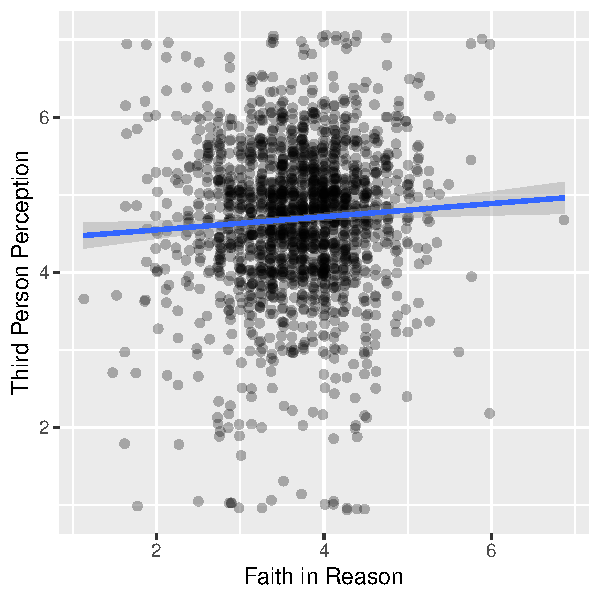
\includegraphics[width=0.75\linewidth]{faithinreason_files/figure-latex/tpe-1} 

}

\caption{Scatterplot of Faith in Reason scores against Third Person Perception score. Note 0.1 jitter applied to x-axes values to allow visualisation of point density}\label{fig:tpe}
\end{figure}

\hypertarget{discussion}{%
\section{Discussion}\label{discussion}}

This paper arose out of a note published online (Stafford, 2022) which we cite for completeness and by way of allowing it to be checked that the intention of the study has been consistent between conceptualisation and publication.

\hypertarget{summary-1}{%
\subsection{Summary}\label{summary-1}}

After developing eight items and gathering responses from a representative sample of UK adults, we assessed dimensionality using conventional factor analysis, Mokken scale analysis (from item response theory) and experimental graph analysis. Conventional factor analysis and Mokken scale analysis suggested that a unidimensional solution was dominant, and six of the items could be used in coherent scale. EGA confirmed that one item - 5 - was least associated with all the others, but also suggested that a items might be grouped into two communities. Exploring the differences, similarities, costs and benefits of EGA for scale analysis is beyond the scope of this report. We note that it affords visual insight into the structure within dimensional groupings of items; showing, here, that item 5 is least associated with the network and item 1 - the item which assesses generic endorsement of the rationality of others - is most central.

We combined items 1,2,3,4,6 and 7 into a single metric - the Faith in Reason scale. Scores on this indicated that a) a large variation exists in beliefs in the rationality or reasonableness of other people (Figure \ref{fig:meanhistogram}) and b) the center of the distribution of these beliefs is slightly away from neutral, reflecting endorsement of the negative sentiment that other people tend to be misinformed, credible and irrational. This stands in contrast to other domains where attitudes have found to be optimistic or beliefs in a just world (Lerner \& Lerner, 1980). It is consonant with a long standing programme fo research into the Third Person Effect.

Scores on the Faith in Reason scale are not determined by education, need for democracy, generalised trust or our specific measure of the Third Person Perception in the context of electoral adverts. Generalised Trust has a moderate association with Faith in Reason, suggesting that they may tap similar underlying beliefs about other people (their trustworthiness and reasonableness). We do not provide any evidence of causal direction, how one set of beliefs may inform the other, nor evidence of how interventions which may affect Faith in Reason, for example, may in turn affect generalised trust. The lack of relation with Third Person Perception is notable, suggesting that domain specific beliefs about susceptibility to influence in a particular context do not strongly link to general beliefs about human reasonableness.

\hypertarget{scale-development}{%
\subsection{scale development}\label{scale-development}}

Issues with scale development and validity testing are usefully reviewed in Flake and Fried (2020); Clark and Watson (2019); Boateng, Neilands, Frongillo, Melgar-Quiñonez, and Young (2018). With the current report we do not pretend to have completed scale development and testing. We merely report the beginnings of the development of a scale for measuring belief in the rationality or reasonableness of the typical citizen.

\hypertarget{wither-misinformation}{%
\subsection{Wither misinformation}\label{wither-misinformation}}

The nature of human rationality is a perenial concern, both in terms of what it means for our self-regard and societal projects like democracy. Recent concerns over misinformation have amplified these concerns, and often assumed a pessimistic view of human credulity and bias. Nonetheless, extensive evidence supports measured optimism about human rationality - that the capacity for due skeptism, warrented trust, and reason responsiveness is widespread (Mercier, 2020; Nyhan, 2020). Responses to our survey appear to reflect these competing currents, with some endorsing extemely pessimistic views of human reason, other endorseing extemely optimistic views, and the majority represented in the middle. It remains to be seen how future world events and the dissemination of empricial results from the cognitive sciences might affect the population level Faith in Reason.

\hypertarget{references}{%
\section*{References}\label{references}}
\addcontentsline{toc}{section}{References}

\hypertarget{refs}{}
\begin{CSLReferences}{1}{0}
\leavevmode\vadjust pre{\hypertarget{ref-rmarkdowncite}{}}%
Allaire, J., Xie, Y., McPherson, J., Luraschi, J., Ushey, K., Atkins, A., \ldots{} Iannone, R. (2020). \emph{Rmarkdown: Dynamic documents for r}. Retrieved from \url{https://github.com/rstudio/rmarkdown}

\leavevmode\vadjust pre{\hypertarget{ref-altay2023}{}}%
Altay, S., \& Acerbi, A. (2023). People believe misinformation is a threat because they assume others are gullible. \emph{New Media \& Society}, 14614448231153379.

\leavevmode\vadjust pre{\hypertarget{ref-aust2020}{}}%
Aust, F., \& Barth, M. (2020). \emph{{papaja}: {Create} {APA} manuscripts with {R Markdown}}. Retrieved from \url{https://github.com/crsh/papaja}

\leavevmode\vadjust pre{\hypertarget{ref-boateng2018}{}}%
Boateng, G. O., Neilands, T. B., Frongillo, E. A., Melgar-Quiñonez, H. R., \& Young, S. L. (2018). Best practices for developing and validating scales for health, social, and behavioral research: A primer. \emph{Frontiers in Public Health}, \emph{6}, 149.

\leavevmode\vadjust pre{\hypertarget{ref-brand2022}{}}%
Brand, C. O., \& Stafford, T. (2022). Using dialogues to increase positive attitudes towards COVID-19 vaccines in a vaccine-hesitant UK population. \emph{Royal Society Open Science}, \emph{9}(10), 220366.

\leavevmode\vadjust pre{\hypertarget{ref-brehm1997}{}}%
Brehm, J., \& Rahn, W. (1997). Individual-level evidence for the causes and consequences of social capital. \emph{American Journal of Political Science}, 999--1023.

\leavevmode\vadjust pre{\hypertarget{ref-chung2016}{}}%
Chung, S., \& Moon, S.-I. (2016). Is the third-person effect real? A critical examination of rationales, testing methods, and previous findings of the third-person effect on censorship attitudes. \emph{Human Communication Research}, \emph{42}(2), 312--337.

\leavevmode\vadjust pre{\hypertarget{ref-clark2019}{}}%
Clark, L. A., \& Watson, D. (2019). Constructing validity: New developments in creating objective measuring instruments. \emph{Psychological Assessment}, \emph{31}(12), 1412.

\leavevmode\vadjust pre{\hypertarget{ref-cohn2019}{}}%
Cohn, A., Maréchal, M. A., Tannenbaum, D., \& Zünd, C. L. (2019). Civic honesty around the globe. \emph{Science}, \emph{365}(6448), 70--73.

\leavevmode\vadjust pre{\hypertarget{ref-davison1983}{}}%
Davison, W. P. (1983). The third-person effect in communication. \emph{Public Opinion Quarterly}, \emph{47}(1), 1--15.

\leavevmode\vadjust pre{\hypertarget{ref-dawson2009}{}}%
Dawson, N. V., \& Gregory, F. (2009). Correspondence and coherence in science: A brief historical perspective. \emph{Judgment and Decision Making}, \emph{4}(2), 126--133.

\leavevmode\vadjust pre{\hypertarget{ref-eiser2009}{}}%
Eiser, J. R., Stafford, T., Henneberry, J., \& Catney, P. (2009). {``Trust me, i'm a scientist (not a developer)''}: Perceived expertise and motives as predictors of trust in assessment of risk from contaminated land. \emph{Risk Analysis: An International Journal}, \emph{29}(2), 288--297.

\leavevmode\vadjust pre{\hypertarget{ref-qgraph}{}}%
Epskamp, S., Cramer, A. O. J., Waldorp, L. J., Schmittmann, V. D., \& Borsboom, D. (2012). {qgraph}: Network visualizations of relationships in psychometric data. \emph{Journal of Statistical Software}, \emph{48}(4), 1--18.

\leavevmode\vadjust pre{\hypertarget{ref-feng2012}{}}%
Feng, G. C., \& Guo, S. Z. (2012). Support for censorship: A multilevel meta-analysis of the third-person effect. \emph{Communication Reports}, \emph{25}(1), 40--50.

\leavevmode\vadjust pre{\hypertarget{ref-flake2020}{}}%
Flake, J. K., \& Fried, E. I. (2020). Measurement schmeasurement: Questionable measurement practices and how to avoid them. \emph{Advances in Methods and Practices in Psychological Science}, \emph{3}(4), 456--465.

\leavevmode\vadjust pre{\hypertarget{ref-furnham1985}{}}%
Furnham, A., Johnson, C., \& Rawles, R. (1985). The determinants of beliefs in human nature. \emph{Personality and Individual Differences}, \emph{6}(6), 675--684.

\leavevmode\vadjust pre{\hypertarget{ref-gss}{}}%
General Social Survey Team. (2023). \emph{General social survey}. Available at: \url{https://gss.norc.org}.

\leavevmode\vadjust pre{\hypertarget{ref-gigerenzer2011}{}}%
Gigerenzer, G., \& Gaissmaier, W. (2011). Heuristic decision making. \emph{Annual Review of Psychology}, \emph{62}, 451--482.

\leavevmode\vadjust pre{\hypertarget{ref-golino2020eganet}{}}%
Golino, H. F., Christensen, A., \& Moulder, R. (2020). EGAnet: Exploratory graph analysis: A framework for estimating the number of dimensions in multivariate data using network psychometrics. \emph{R Package Version 0.9}, \emph{2}.

\leavevmode\vadjust pre{\hypertarget{ref-golino2020investigating}{}}%
Golino, H. F., Shi, D., Christensen, A. P., Garrido, L. E., Nieto, M. D., Sadana, R., \ldots{} Martinez-Molina, A. (2020). Investigating the performance of exploratory graph analysis and traditional techniques to identify the number of latent factors: A simulation and tutorial. \emph{Psychological Methods}, \emph{25}(3), 292.

\leavevmode\vadjust pre{\hypertarget{ref-EGAnet}{}}%
Golino, H., \& Christensen, A. P. (2022). \emph{EGAnet: Exploratory graph analysis -- a framework for estimating the number of dimensions in multivariate data using network psychometrics}.

\leavevmode\vadjust pre{\hypertarget{ref-hoes2022}{}}%
Hoes, E., Clemm von Hohenberg, B., Gessler, T., Wojcieszak, M., \& Qian, S. (2022). \emph{The cure worse than the disease? How the media's attention to misinformation decreases trust}. PsyArXiv. \url{https://doi.org/10.31234/osf.io/4m92p}

\leavevmode\vadjust pre{\hypertarget{ref-holcombe2020documenting}{}}%
Holcombe, A. O., Kovacs, M., Aust, F., \& Aczel, B. (2020). Documenting contributions to scholarly articles using CRediT and tenzing. \emph{PLoS One}, \emph{15}(12), e0244611.

\leavevmode\vadjust pre{\hypertarget{ref-wvs}{}}%
Inglehart, C., R., \& Team, W. (2023). \emph{World values survey}. Available at: \url{https://www.worldvaluessurvey.org}.

\leavevmode\vadjust pre{\hypertarget{ref-jungherr2022}{}}%
Jungherr, A., \& Rauchfleisch, A. (2022). \emph{Negative downstream effects of disinformation discourse: Evidence from the US}. SocArXiv.

\leavevmode\vadjust pre{\hypertarget{ref-kahneman1982}{}}%
Kahneman, D., Slovic, S. P., \& Tversky, A. (1982). \emph{Judgment under uncertainty: Heuristics and biases}. Cambridge university press.

\leavevmode\vadjust pre{\hypertarget{ref-karadzhov2022}{}}%
Karadzhov, G., Stafford, T., \& Vlachos, A. (2022). What makes you change your mind? An empirical investigation in online group decision-making conversations. \emph{arXiv Preprint arXiv:2207.12035}.

\leavevmode\vadjust pre{\hypertarget{ref-karpf2019}{}}%
Karpf, D. (2019). On digital disinformation and democratic myths. Retrieved from \url{https://mediawell.ssrc.org/expert-reflections/on-digital-disinformation-and-democratic-myths/}

\leavevmode\vadjust pre{\hypertarget{ref-lee2021}{}}%
Lee, T. (2021). How people perceive influence of fake news and why it matters. \emph{Communication Quarterly}, \emph{69}(4), 431--453.

\leavevmode\vadjust pre{\hypertarget{ref-lerner1980belief}{}}%
Lerner, M. J., \& Lerner, M. J. (1980). \emph{The belief in a just world}. Springer.

\leavevmode\vadjust pre{\hypertarget{ref-lyons2022}{}}%
Lyons, B. A. (2022). Why we should rethink the third-person effect: Disentangling bias and earned confidence using behavioral data. \emph{Journal of Communication}, \emph{72}(5), 565--577.

\leavevmode\vadjust pre{\hypertarget{ref-mercier2020}{}}%
Mercier, H. (2020). \emph{Not born yesterday}. Princeton: Princeton University Press.

\leavevmode\vadjust pre{\hypertarget{ref-mercier2011}{}}%
Mercier, H., \& Sperber, D. (2011). Why do humans reason? Arguments for an argumentative theory. \emph{Behavioral and Brain Sciences}, \emph{34}(2), 57--74.

\leavevmode\vadjust pre{\hypertarget{ref-here}{}}%
Müller, K. (2020). \emph{Here: A simpler way to find your files}. Retrieved from \url{https://CRAN.R-project.org/package=here}

\leavevmode\vadjust pre{\hypertarget{ref-nisbet2021}{}}%
Nisbet, E. C., Mortenson, C., \& Li, Q. (2021). The presumed influence of election misinformation on others reduces our own satisfaction with democracy. \emph{Harvard Kennedy School Misinformation Review}.

\leavevmode\vadjust pre{\hypertarget{ref-nisbett1977}{}}%
Nisbett, R. E., \& Wilson, T. D. (1977). Telling more than we can know: Verbal reports on mental processes. \emph{Psychological Review}, \emph{84}(3), 231.

\leavevmode\vadjust pre{\hypertarget{ref-nyhan2020facts}{}}%
Nyhan, B. (2020). Facts and myths about misperceptions. \emph{Journal of Economic Perspectives}, \emph{34}(3), 220--236.

\leavevmode\vadjust pre{\hypertarget{ref-olshansky2020}{}}%
Olshansky, A., \& Landrum, A. R. (2020). Third-person perceptions and calls for censorship of flat earth videos on YouTube. \emph{Media and Communication}, \emph{8}(2), 387--400.

\leavevmode\vadjust pre{\hypertarget{ref-pascal1910}{}}%
Pascal, B. (1669/1910). \emph{Thoughts} (Vol. 48). PF Collier \& son. Retrieved from \url{\%22http://entersection.com/posts/1189-blaise-pascal-on-man-as-a-thinking-reed\%22}

\leavevmode\vadjust pre{\hypertarget{ref-paxton1999}{}}%
Paxton, P. (1999). Is social capital declining in the united states? A multiple indicator assessment. \emph{American Journal of Sociology}, \emph{105}(1), 88--127.

\leavevmode\vadjust pre{\hypertarget{ref-perloff2002}{}}%
Perloff, R. M. (2002). The third-person effect. In \emph{Media effects} (pp. 499--516). Routledge.

\leavevmode\vadjust pre{\hypertarget{ref-putnam2000}{}}%
Putnam, R. D. (2000). \emph{Bowling alone: The collapse and revival of american community}. Simon; schuster.

\leavevmode\vadjust pre{\hypertarget{ref-psych}{}}%
Revelle, W. (2022). \emph{Psych: Procedures for psychological, psychometric, and personality research}. Evanston, Illinois: Northwestern University. Retrieved from \url{https://CRAN.R-project.org/package=psych}

\leavevmode\vadjust pre{\hypertarget{ref-ltm}{}}%
Rizopoulos, D. (2006). Ltm: An r package for latent variable modelling and item response theory analyses. \emph{Journal of Statistical Software}, \emph{17}(5), 1--25. Retrieved from \url{https://doi.org/10.18637/jss.v017.i05}

\leavevmode\vadjust pre{\hypertarget{ref-samuels2002}{}}%
Samuels, R., Stich, S., \& Bishop, M. (2002). {236Ending the Rationality Wars How to Make Disputes about Human Rationality Disappear}. In \emph{{Common Sense, Reasoning, and Rationality}}. Oxford University Press. \url{https://doi.org/10.1093/0195147669.003.0011}

\leavevmode\vadjust pre{\hypertarget{ref-sijtsma2017tutorial}{}}%
Sijtsma, K., \& Ark, L. A. van der. (2017). A tutorial on how to do a mokken scale analysis on your test and questionnaire data. \emph{British Journal of Mathematical and Statistical Psychology}, \emph{70}(1), 137--158.

\leavevmode\vadjust pre{\hypertarget{ref-sommer2022}{}}%
Sommer, J., Musolino, J., \& Hemmer, P. (2022). A hobgoblin of large minds: Troubles with consistency in belief. \emph{Wiley Interdisciplinary Reviews: Cognitive Science}, e1639.

\leavevmode\vadjust pre{\hypertarget{ref-stafford2014}{}}%
Stafford, T. (2014). The perspectival shift: How experiments on unconscious processing don't justify the claims made for them. \emph{Frontiers in Psychology}, \emph{5}, 1067. \url{https://doi.org/10.3389/fpsyg.2014.01067}

\leavevmode\vadjust pre{\hypertarget{ref-stafford2020evidence}{}}%
Stafford, T. (2020). Evidence for the rationalisation phenomenon is exaggerated. \emph{Behavioral and Brain Sciences}, \emph{43}.

\leavevmode\vadjust pre{\hypertarget{ref-stafford2022}{}}%
Stafford, T. (2022, May 8). Quantifying our faith in reason. Retrieved from \url{https://tomstafford.substack.com/p/quantifying-our-faith-in-reason}

\leavevmode\vadjust pre{\hypertarget{ref-stavrova2016}{}}%
Stavrova, O., \& Ehlebracht, D. (2016). Cynical beliefs about human nature and income: Longitudinal and cross-cultural analyses. \emph{Journal of Personality and Social Psychology}, \emph{110}(1), 116.

\leavevmode\vadjust pre{\hypertarget{ref-stojanov2020}{}}%
Stojanov, A., Bering, J. M., \& Halberstadt, J. (2020). Does perceived lack of control lead to conspiracy theory beliefs? Findings from an online MTurk sample. \emph{PLoS One}, \emph{15}(8), e0237771.

\leavevmode\vadjust pre{\hypertarget{ref-stojanov2019}{}}%
Stojanov, A., \& Halberstadt, J. (2019). The conspiracy mentality scale. \emph{Social Psychology}, \emph{50}, 215-\/-232. \url{https://doi.org/10.1027/1864-9335/a000381}

\leavevmode\vadjust pre{\hypertarget{ref-sun2008}{}}%
Sun, Y., Pan, Z., \& Shen, L. (2008). Understanding the third-person perception: Evidence from a meta-analysis. \emph{Journal of Communication}, \emph{58}(2), 280--300.

\leavevmode\vadjust pre{\hypertarget{ref-swami2017}{}}%
Swami, V., Barron, D., Weis, L., Voracek, M., Stieger, S., \& Furnham, A. (2017). An examination of the factorial and convergent validity of four measures of conspiracist ideation, with recommendations for researchers. \emph{PloS One}, \emph{12}(2), e0172617.

\leavevmode\vadjust pre{\hypertarget{ref-mokken}{}}%
Van der Ark, L. A. (2007). Mokken scale analysis in {R}. \emph{Journal of Statistical Software}, \emph{20}(11), 1--19. Retrieved from \url{https://www.jstatsoft.org/article/view/v020i11}

\leavevmode\vadjust pre{\hypertarget{ref-corrtable}{}}%
van der Laken, P. (2022). \emph{Corrtable: Creates and saves out a correlation table with significance levels indicated}. Retrieved from \url{https://CRAN.R-project.org/package=corrtable}

\leavevmode\vadjust pre{\hypertarget{ref-van2011ordinal}{}}%
Van Schuur, W. H. (2011). \emph{Ordinal item response theory: Mokken scale analysis}. Sage.

\leavevmode\vadjust pre{\hypertarget{ref-tidyverse}{}}%
Wickham, H., Averick, M., Bryan, J., Chang, W., McGowan, L. D., François, R., \ldots{} Yutani, H. (2019). Welcome to the {tidyverse}. \emph{Journal of Open Source Software}, \emph{4}(43), 1686. \url{https://doi.org/10.21105/joss.01686}

\leavevmode\vadjust pre{\hypertarget{ref-knitr}{}}%
Xie, Y. (2022). \emph{Knitr: A general-purpose package for dynamic report generation in r}. Retrieved from \url{https://yihui.org/knitr/}

\leavevmode\vadjust pre{\hypertarget{ref-zhu2023}{}}%
Zhu, J., Dommett, K., \& Stafford, T. (submitted). \emph{What makes online political ads unacceptable? Interrogating public attitudes to inform regulatory responses}.

\end{CSLReferences}


\end{document}
